\subsection{From Skill Access to Usable Teaching Artifacts}
\label{sec:access}
\label{sec:cases}

The native interface exposes the task's designated educational package;
the agent decides whether to load it. We count a completed call naming that
package, requiring returned content for locally available raw traces and
using completed-call summaries where those are the retained evidence.
Missing captures remain unknown. GLM-5.3 is excluded from this access
analysis because its retained answers span two exposure modes
(Appendix~\ref{app:execution}).

\begin{figure*}[t]
\centering
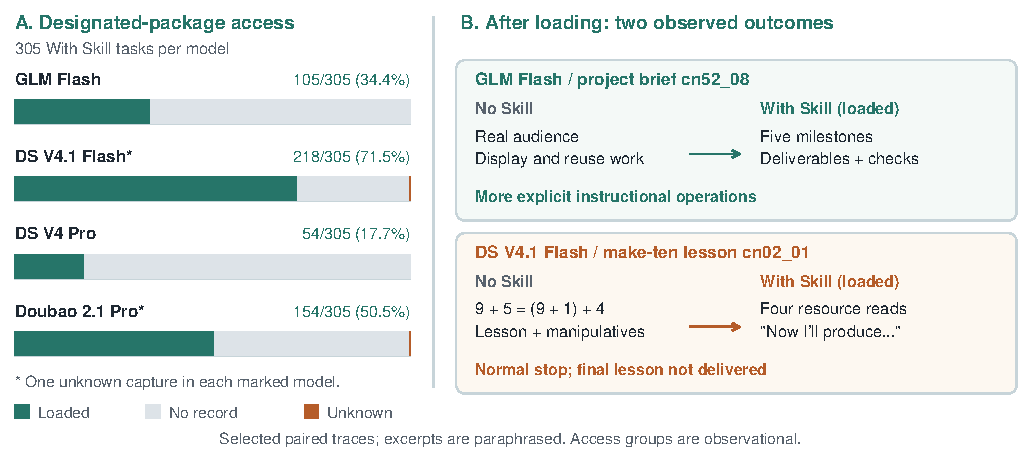
\includegraphics[width=\textwidth]{figures/access_artifacts_v41.pdf}
\caption{From package availability to teaching artifacts. Left: observed
access among 305 With tasks per model; unknown captures are separate from
no recorded access. Right: paraphrased paired artifacts show explicit project
milestones after loading, but a lesson that ends as a promise rather than a
deliverable. Cases illustrate mechanisms, not prevalence or a causal effect
of loading. Full subgroup results appear in Appendix~\ref{app:inventory}.}
\label{fig:access-artifacts}
\end{figure*}

\paragraph{Availability does not guarantee access.}
Figure~\ref{fig:access-artifacts} records 531 loads over 1,220 With tasks, ranging
from Pro's 17.70\% to DeepSeek Flash's 71.48\%. Every recorded educational
load names the designated package. With one task-scoped educational candidate,
this measures the decision to access relevant guidance; it does not test
retrieval among all 14 Skills. Loaded common-valid groups improve for GLM
Flash, Pro, and Doubao, but decline for DeepSeek Flash. Since agents choose
whether to load and the resulting groups differ in task composition, these
associations do not identify a causal loading effect.

\paragraph{A useful procedure makes classroom operations explicit.}
In GLM Flash's project-brief task \texttt{cn52\_08}, the teacher has no
budget or laboratory and wants student projects with a real audience. Both
answers identify meaningful uses for the work. After loading the package,
the With answer additionally organizes five milestones, stage-specific
deliverables, explicit instruction, and completion checkpoints. This is
observable procedural uptake beyond mentioning the Skill. Judged candidate quality
$J$ rises from 0.856 to 0.912, although the reference component also falls
from 0.918 to 0.806; the resulting $+4.83$ relative-score change therefore
cannot be assigned entirely to the candidate's improvement.

\paragraph{Successful access can still end without a deliverable.}
For DeepSeek Flash's lesson-building task \texttt{cn02\_01}, No Skill
provides a concrete make-ten lesson with manipulatives and fallback materials.
With Skill loads the package and four resources, but terminates with a
promise to produce materials instead of the lesson itself. The answer has
a normal stop and a zero candidate component. More broadly, DeepSeek Flash
has 60 failed supporting-file reads over 49 tasks despite successful main
package loads. These records distinguish access, resource execution, and
final delivery. Our 32 exported paired cases connect those stages to actual
teaching products; they were selected diagnostically and do not estimate
failure prevalence (Appendix~\ref{app:inventory}).
